% ****** Start of file apssamp.tex ******
%
%   This file is part of the APS files in the REVTeX 4.2 distribution.
%   Version 4.2a of REVTeX, December 2014
%
%   Copyright (c) 2014 The American Physical Society.
%
%   See the REVTeX 4 README file for restrictions and more information.
%
% TeX'ing this file requires that you have AMS-LaTeX 2.0 installed
% as well as the rest of the prerequisites for REVTeX 4.2
%
% See the REVTeX 4 README file
% It also requires running BibTeX. The commands are as follows:
%
%  1)  latex apssamp.tex
%  2)  bibtex apssamp
%  3)  latex apssamp.tex
%  4)  latex apssamp.tex
%
\documentclass[%
 reprint,
superscriptaddress,
%groupedaddress,
%unsortedaddress,
%runinaddress,
%frontmatterverbose, 
%preprint,
%preprintnumbers,
%nofootinbib,
%nobibnotes,
%bibnotes,
 amsmath,amssymb,
 aps,
%pra,
%prb,
%rmp,
%prstab,
%prstper,
%floatfix,
]{revtex4-2}

\usepackage{graphicx}% Include figure files
\usepackage{dcolumn}% Align table columns on decimal point
\usepackage{xcolor}
\usepackage{bm}% bold math
%\usepackage{hyperref}% add hypertext capabilities
%\usepackage[mathlines]{lineno}% Enable numbering of text and display math
%\linenumbers\relax % Commence numbering lines

%\usepackage[showframe,%Uncomment any one of the following lines to test 
%%scale=0.7, marginratio={1:1, 2:3}, ignoreall,% default settings
%%text={7in,10in},centering,
%%margin=1.5in,
%%total={6.5in,8.75in}, top=1.2in, left=0.9in, includefoot,
%%height=10in,a5paper,hmargin={3cm,0.8in},
%]{geometry}

\begin{document}

\title{Modeling the Spread of Ebola in West Africa} % Force line breaks with \\

\author{Jason Hunter}
% UNCOMMENT THIS IF YOU HAVE A SECOND AUTHOR
% \author{Second Author}


\date{December 15, 2024}% It is always \today, today,
             %  but any date may be explicitly specified

\begin{abstract}
{\bf Abstract:} \textcolor{blue}{For this project, I designed and created a standard SIR model to simulate the spread of Ebola in a population. From the standard SIR model, I created a modified model to attempt to tune the model to Ebola specific dynamics. This model accounted for an additional population of 'exposed' individuals, which made it possible to take into account the latency period of Ebola. Finally, I added a quarantine parameter to the model to simulate the effects of containment on the spread of the disease. The model was then used to simulate the spread of Ebola in West Africa using a mixture of both mock data and real metrics gathered from various datasets. I then attempt to do a more geospatial analysis of the epidemic as it took place in West Africa.}
\end{abstract}

\maketitle

\section{Introduction and Background}

You can refer to items in your bibliography in this section, too using LaTeX's citations \cite{aa} and \cite{bb}.

\textcolor{blue}{ Ebola virus disease (EVD) is a highly lethal viral hemmorhagic fever which has caused several widespread outbreaks in Africa. It was first discovered in 1976 when two outbreaks occurred in Sudan and the Democratic Republic of Congo near the Ebola river, debuting the disease's name. Since then the disease has caused several outbreaks in Africa, with the most severe being the 2014-2016 outbreak. 
The virus is zoonotic in nature, meaning that it spreads from wild animals to humans. It is widely believed that fruit bats are the source of the virus, and may have been sold as bushmeat at local markets. The virus then spreads through human-to-human contact, and can be spread through bodily fluids, blood, and other secretions. 
The virus has an incubation period in the range of 2-21 days, and symptoms include fever, muscle pain, fatigue, headache, and sore throat. These symptoms are then followed by vomiting, diarrhea, rash, and in some cases, internal and external bleeding. The disease has a high mortality rate, with the 2014-2016 outbreak in West Africa having an average mortality rate of around 40\%, resulting in around 11,000 deaths out of about 28,000 cases across Sierra Leone, Liberia, and Guinea.}

\textcolor{blue}{A common model used in the simulation of infectious disease spread is the SIR model. This model separates the population into four distinct compartments: Susceptible, Infected, and Recovered. A set of differential equations is then used to model the flow of individuals between these populations with respect to time. A common extension to the SIR model is the SEIR model, which adds an additional compartment for Exposed individuals. 
This compartment accounts for the latency period of the disease, where individuals are infected but not yet infectious. This is especially useful for diseases such as Ebola, which have an extensive latent period. When combined with realistic disease parameters and population data, these models can be used to simulate the spread of infectious diseases and predict the effects of various interventions.}

\textcolor{blue}{In my project, I've used a modified SEIR model in an attempt to run simulations of the spread of Ebola in West Africa. My modifications to the model include the addition of a containment parameter, which effectively acts as a quarantine for infected people. Alongside this, I've also added an effectiveness rate to the containment parameter, which allows for the simulation of different levels of containment. 
With this I hope to better understand how a combination of both rapid and effective containment procedures can help to mitigate the spread of contagious disease.}

\textcolor{blue}{I've also gathered data from a variety of sources, including the World Health Organization (WHO), the Centers for Disease Control and Prevention (CDC), as well as a few githubs. This data includes Ebola specific disease metrics, as well as coordinates of the affected areas. I then use this data to attempt a geospatial analysis of the epidemic as it took place in West Africa.}

\section{Learning Goals}

\textcolor{blue}{My main learning goal for this project was to model the spread of the Ebola epidemic in West African countries using an SEIR framework and to understand how containment measures could have affected the spread of the disease. I aimed to use this SEIR model to visualize the spread of the disease in a way that would be easy to understand and interpret. I wanted to gain a better understanding of how these models work, and how they are used to represent real-world disease dynamics.}

\textcolor{blue}{I also gained vital experience in both data collection and analysis during this project. It was important to source data from several places, and to understand the importance of using clean and reliable data. I also learned how to use this data to create visualizations that could help to better understand the spread of the disease. This continued to excel my skills in Python and data analysis.
I learned how to use geospatial data to create maps of the spread of the disease, and how to use these maps to better understand the spread of the disease. This was a new skill for me, and I found it to be very interesting and useful.}

\section{Findings and Results}

What did you find? Use subsections to explain what you did and what you found. 

\begin{figure}[t]
    \centering
    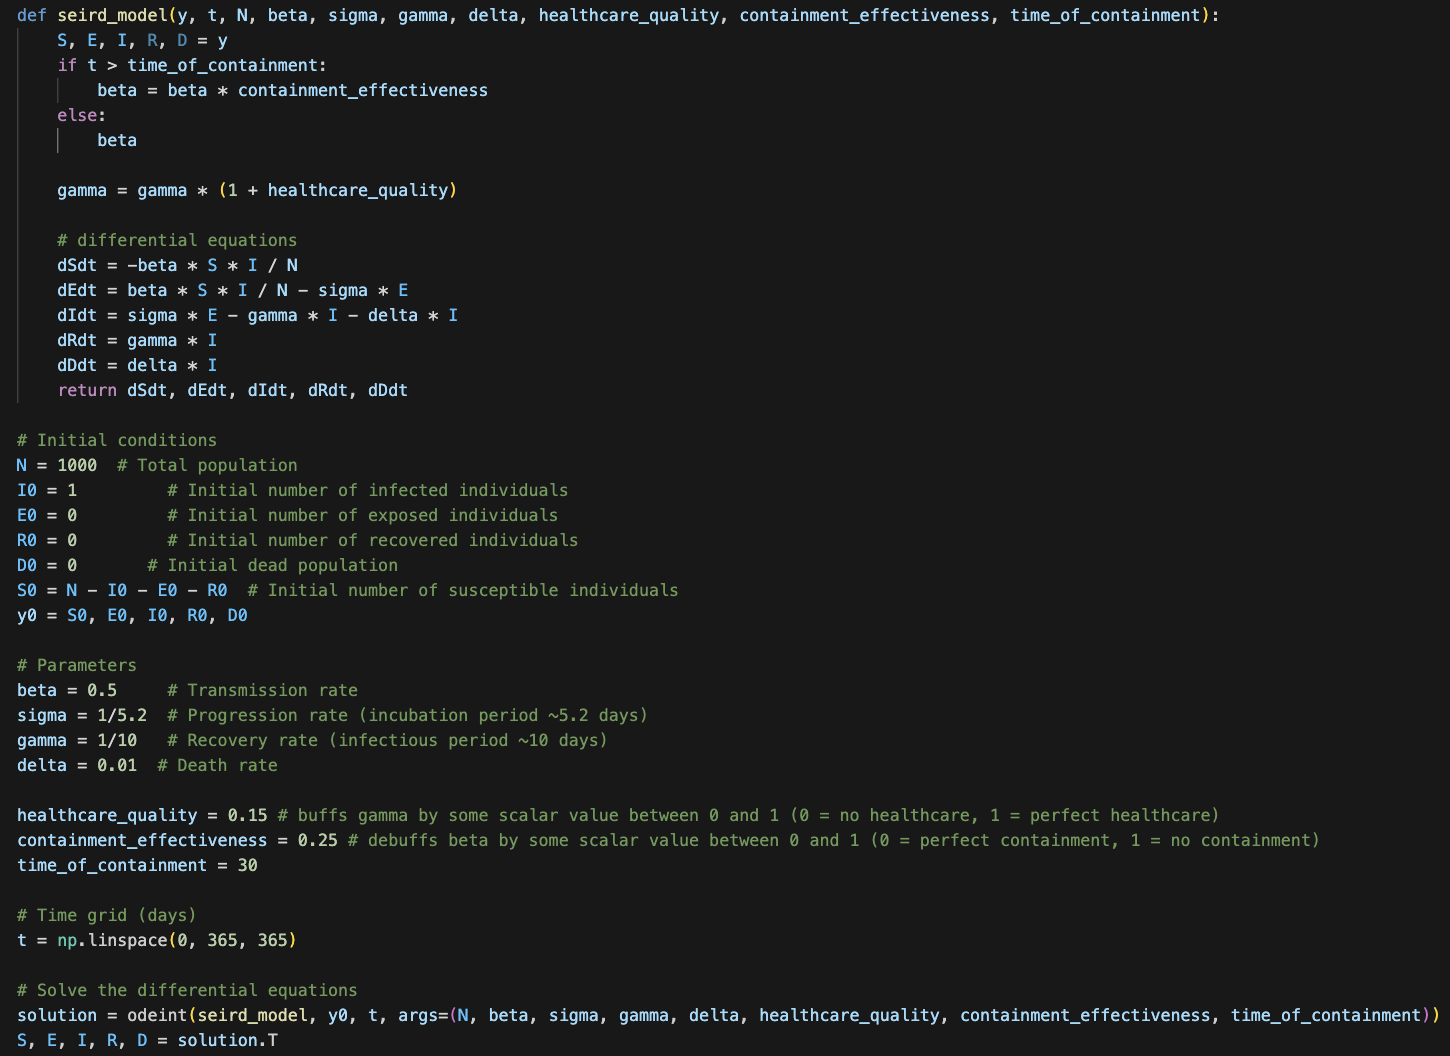
\includegraphics[width=0.5\textwidth]{SEIRD Model.png}
    \caption{Python code for the SEIR model used in this project.}
    \label{SEIR Model}
\end{figure}

\textcolor{blue}{Using the SEIR model depicted in Figure \ref{SEIR Model}, I was able to run simulations on the progression of Ebola outbreaks in countries in West Africa. I included key parameters that are a part of all SEIR models, such as the transmission rate $\beta$, which dictates the rate at which susceptible individuals become infected, the rate of recovery $\gamma$, which is the rate at which infectious individuals recover, as well as the incubation rate $\sigma$, which is indicative of the rate at which exposed individuals become infectious.
I also include a death rate $\delta$, which is the rate at which infected individuals die. This is an important parameter for diseases such as Ebola, which have a high mortality rate.
Lastly, I included two parameters for containment: the date at which containment measures were implemented, and the effectiveness of these measures.}
\textcolor{blue}{The SEIR equations used in the model are as follows:
\begin{equation}
    \frac{dS}{dt} = -\beta \frac{S}{N} I
    \label{dSdt}
\end{equation}
\begin{equation}
    \frac{dE}{dt} = \beta \frac{S}{N} I - \sigma E
    \label{dEdt}
\end{equation}
\begin{equation}
    \frac{dI}{dt} = \sigma E - \gamma I - \delta I
    \label{dIdt}
\end{equation}
\begin{equation}
    \frac{dR}{dt} = \gamma I
    \label{dRdt}
\end{equation}
\begin{equation}
    \frac{dD}{dt} = \delta I
    \label{dDdt}
\end{equation}
where $S$ is the number of susceptible individuals, $E$ is the number of exposed individuals, $I$ is the number of infected individuals, $R$ is the number of recovered individuals, $D$ is the number of deceased individuals, $N$ is the total population, $\beta$ is the transmission rate, $\sigma$ is the incubation rate, $\gamma$ is the recovery rate, and $\delta$ is the death rate.}

\textcolor{blue}{At this point I ran several simulations to try to understand how turning these various knobs on the model would affect the spread of the disease.}

\subsection{Impact of Healthcare Quality}
\textcolor{blue}{An additional parameter I attempted to account for in my model was the quality of healthcare in the affected areas. I added healthcare quality, which was represented as a proportion from 0 to 1, in which 0 represented no healthcare at all and 1 represented the best healthcare possible. This was multiplied by the recovery rate $\gamma$ to simulate the effects of healthcare on the recovery of infected individuals.
In this simulation, I used a healthcare quality of 0.5, a transmission rate of 0.4, a recovery rate of 0.1, an incubation rate of 0.1, and an initial death rate of 0.05, an initial population $N$ of 100, an initial number of infected individuals $I$ of 1, and all other initial compartments set to 0. Additionally, I set the containment effectiveness to 0.5, and the containment date to 30 days after the start of the simulation which runs for a total of 180 days.
\begin{figure}[hbt!]
    \centering
    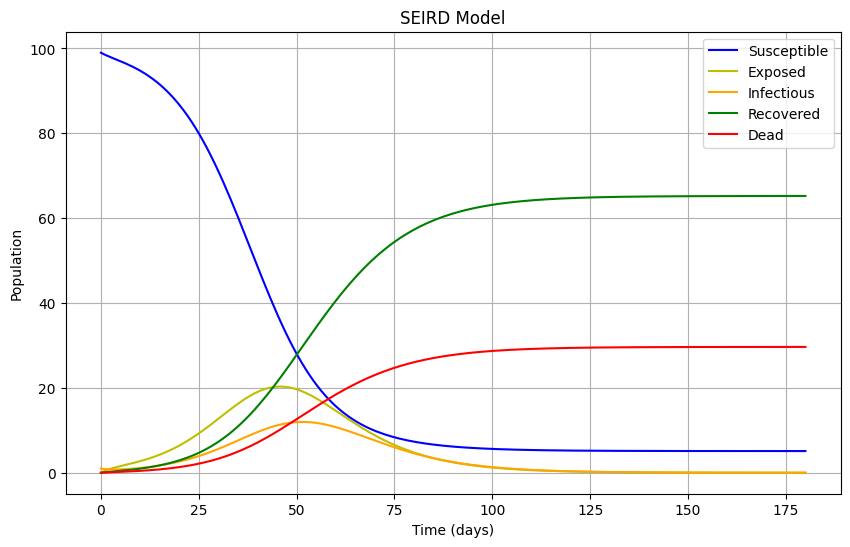
\includegraphics[width=0.5\textwidth]{HealthcareA.png}
    \caption{Simulation w/ Healthcare Quality = 0.5.}
    \label{HealthcareA}
\end{figure}
\begin{figure}[hbt!]
    \centering
    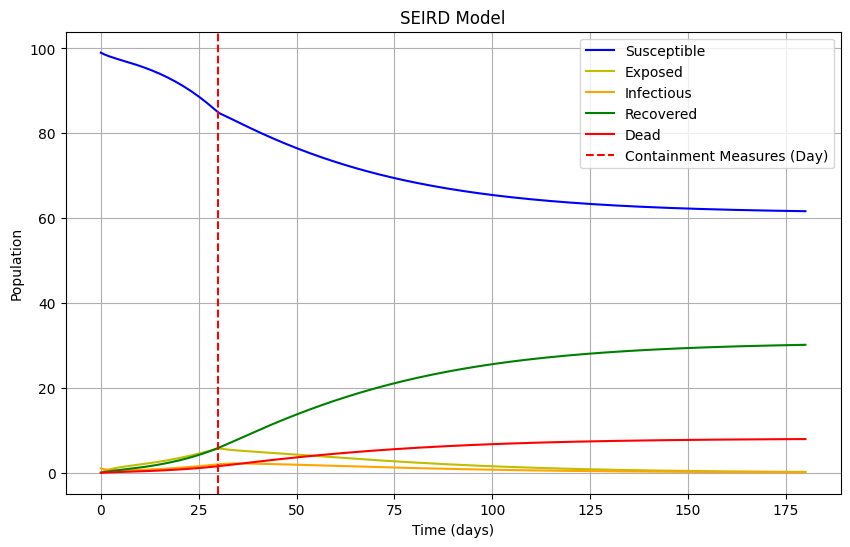
\includegraphics[width=0.5\textwidth]{HealthcareB.png}
    \caption{Simulation w/ Healthcare Quality = 0.9.}
    \label{HealthcareB}
\end{figure}
\begin{figure}[hbt!]
    \centering
    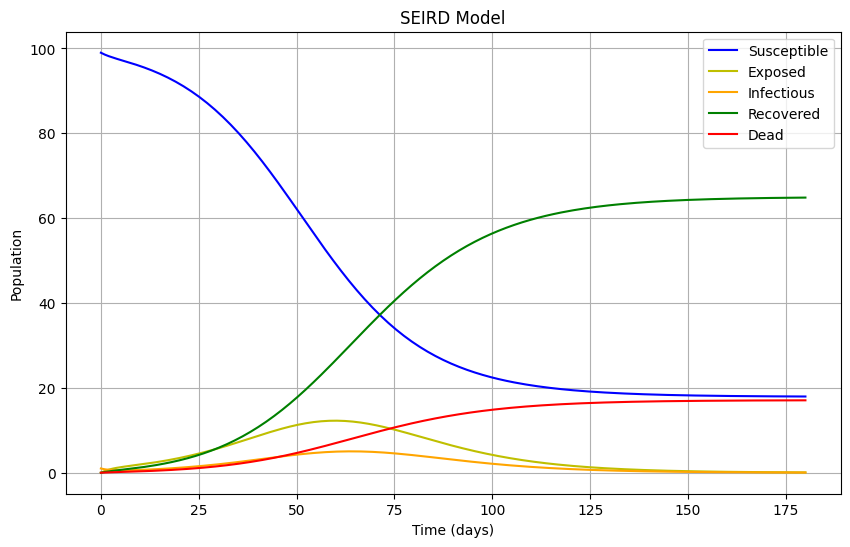
\includegraphics[width=0.5\textwidth]{HealthcareC.png}
    \caption{Simulation w/ Healthcare Quality = 0.1.}
    \label{HealthcareC}
\end{figure} \\
In the model, I found that the quality of healthcare had a significant impact on the spread of the disease. In areas with poor healthcare, the disease spread more rapidly and had a higher mortality rate. In areas with better healthcare, the disease spread more slowly and had a lower mortality rate. This was an important finding, as it highlighted the importance of healthcare in controlling the spread of infectious diseases. }

\subsection{Impact of Containment Measures}
\textcolor{blue}{I also ran simulations to understand the impact of containment measures on the spread of the disease. I used the same parameters as in the previous simulation, but changed the containment effectiveness to 0.9, and the containment date to 30 days after the start of the simulation. I ran the simulation for a total of 180 days.}
\begin{figure}[hbt!]
    \centering
    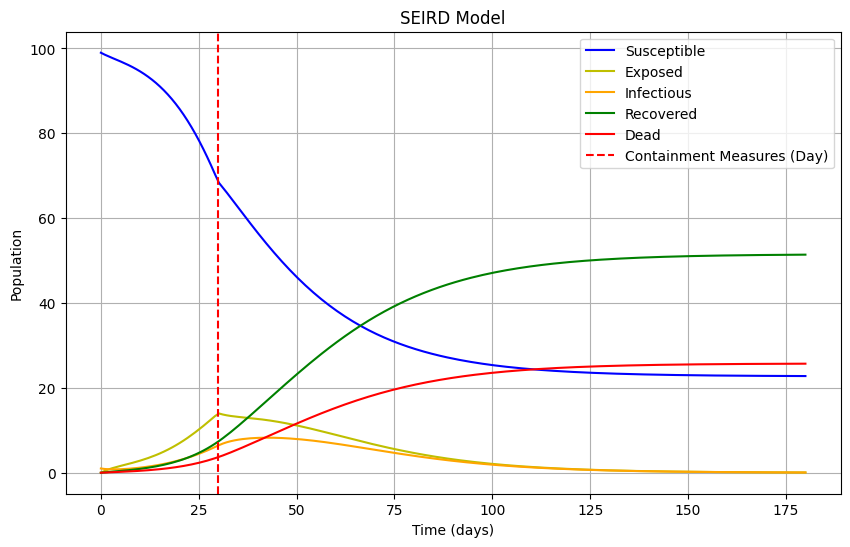
\includegraphics[width=0.5\textwidth]{ContainmentA.png}
    \caption{Simulation w/ Containment Effectiveness = 0.9.}
    \label{ContainmentA}
\end{figure}
\begin{figure}
    \centering
    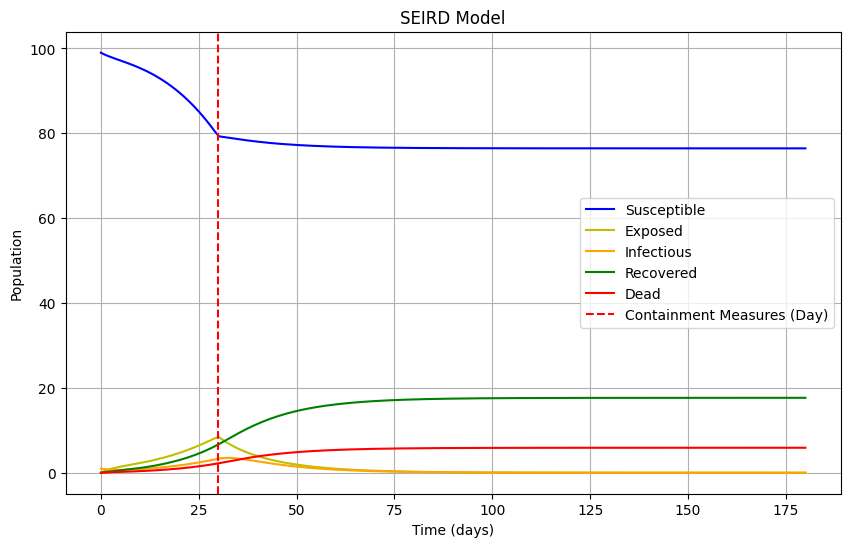
\includegraphics[width=0.5\textwidth]{ContainmentB.png}
    \caption{Simulation w/ Containment Effectiveness = 0.5.}
    \label{ContainmentB}
\end{figure}
\begin{figure}
    \centering
    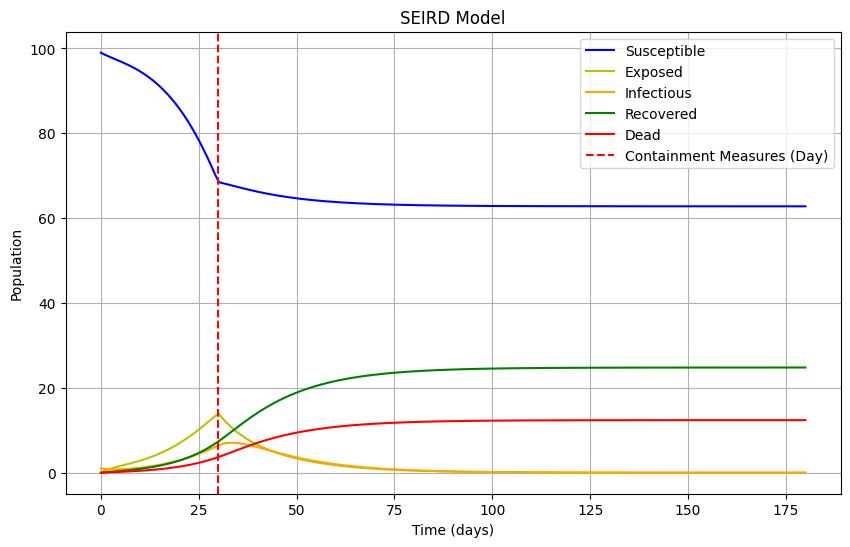
\includegraphics[width = 0.5\textwidth]{ContainmentC.png}
    \caption{Simulation w/ Containment Effectiveness = 0.1.}
    \label{ContainmentC}
\end{figure}

\section{Discussion and Conclusions}

Start by summarizing the key points from your findings and results. Imagine someone who didn't have time to read the whole Results section but wanted to understand what you did. {\it That} is paragraph one.

Dig into some of the results and put them into a broader context. Discuss your results and findings here, in the context of the background that you introduced us to on the first page. Those are your next paragraphs.

Then, reflect: How did your project achieve or not achieve your learning goals?

Finally: Which of your findings surprised you? What were your favorite discoveries and why? 

\textcolor{blue}{Egestas congue quisque egestas diam in arcu cursus euismod quis. Posuere ac ut consequat semper. In nibh mauris cursus mattis molestie a iaculis at erat. Ac orci phasellus egestas tellus rutrum tellus. Sed augue lacus viverra vitae congue eu consequat ac felis. Vivamus arcu felis bibendum ut tristique et egestas quis ipsum. Nunc mattis enim ut tellus. Aliquam purus sit amet luctus venenatis. Amet dictum sit amet justo donec. Hac habitasse platea dictumst quisque. Feugiat scelerisque varius morbi enim nunc faucibus a. Nunc consequat interdum varius sit amet. Sollicitudin aliquam ultrices sagittis orci a scelerisque. Gravida cum sociis natoque penatibus et. Massa ultricies mi quis hendrerit dolor magna eget est. Lectus quam id leo in vitae turpis massa sed elementum. In fermentum posuere urna nec tincidunt praesent semper. Est placerat in egestas erat imperdiet sed. Amet tellus cras adipiscing enim eu. In fermentum et sollicitudin ac orci phasellus egestas tellus.}



\textcolor{blue}{Egestas congue quisque egestas diam in arcu cursus euismod quis. Posuere ac ut consequat semper. In nibh mauris cursus mattis molestie a iaculis at erat. Ac orci phasellus egestas tellus rutrum tellus. Sed augue lacus viverra vitae congue eu consequat ac felis. Vivamus arcu felis bibendum ut tristique et egestas quis ipsum. Nunc mattis enim ut tellus. Aliquam purus sit amet luctus venenatis. Amet dictum sit amet justo donec. Hac habitasse platea dictumst quisque. Feugiat scelerisque varius morbi enim nunc faucibus a. Nunc consequat interdum varius sit amet. Sollicitudin aliquam ultrices sagittis orci a scelerisque. Gravida cum sociis natoque penatibus et. Massa ultricies mi quis hendrerit dolor magna eget est. Lectus quam id leo in vitae turpis massa sed elementum. In fermentum posuere urna nec tincidunt praesent semper. Est placerat in egestas erat imperdiet sed. Amet tellus cras adipiscing enim eu. In fermentum et sollicitudin ac orci phasellus egestas tellus.}

\section{Outlook and Future Work}

Suppose you had another 3 months to work on this project. What further questions would you ask, and why? What would an extended version of this project consider? 

\textcolor{blue}{Egestas congue quisque egestas diam in arcu cursus euismod quis. Posuere ac ut consequat semper. In nibh mauris cursus mattis molestie a iaculis at erat. Ac orci phasellus egestas tellus rutrum tellus. Sed augue lacus viverra vitae congue eu consequat ac felis. Vivamus arcu felis bibendum ut tristique et egestas quis ipsum. Nunc mattis enim ut tellus. Aliquam purus sit amet luctus venenatis. Amet dictum sit amet justo donec. Hac habitasse platea dictumst quisque. Feugiat scelerisque varius morbi enim nunc faucibus a. Nunc consequat interdum varius sit amet. Sollicitudin aliquam ultrices sagittis orci a scelerisque. Gravida cum sociis natoque penatibus et. Massa ultricies mi quis hendrerit dolor magna eget est. Lectus quam id leo in vitae turpis massa sed elementum. In fermentum posuere urna nec tincidunt praesent semper. Est placerat in egestas erat imperdiet sed. Amet tellus cras adipiscing enim eu. In fermentum et sollicitudin ac orci phasellus egestas tellus.}


\begin{thebibliography}{2}

\bibitem{aa} Anna Anderegg, 2019, Thoughts.

\bibitem{bb} Brenda Bradshaw, 2018, Worries.

\end{thebibliography}


\end{document}
%
% ****** End of file apssamp.tex ******
